\documentclass[11pt,a4paper,oneside]{article}

%---- Preamble ----%
\usepackage[utf8]{inputenc}
\usepackage{amsmath}
\usepackage{amsfonts}
\usepackage{amssymb}
\usepackage{graphicx}
\usepackage{parskip} 									
\usepackage[left=2cm,right=2cm,top=2cm,bottom=2cm]{geometry}
\usepackage[]{ccicons}
\usepackage{hyperref}
\usepackage{pdfpages}									% add in pdf pages
\usepackage{pdflscape}									% easy landscape pages

\hypersetup{colorlinks,citecolor=black,filecolor=black,linkcolor=black,urlcolor=black}  % TOC hyperlinks

\author{Jamie D. Wilson \\ (wilson.jamied@gmail.com)}
\title{\LaTeX-HowTo}


%---- Document ----%
\begin{document}
\maketitle

\begin{center}
\ccLogo \ccAttribution \ccShareAlike
\end{center}

\tableofcontents

\newpage

\section{Introduction}

This How-To document is designed as a basic introduction for the Earth and Ocean Sciences \LaTeX{} Thesis template, particularly if you've never used or heard of \LaTeX{} before! The idea for the template is to have a freely available, simple starting point for a thesis. You can just copy over your text and make a decent looking thesis already or, if you want, adapt it to what you want.  If you want to adapt the template, the hope is that you can also update the template for future use. 

\LaTeX{} is a little different to making a document in Word.  Essentially, you make a text file that has the content of your thesis interspersed with typed instructions on how to format the text\footnote{You can look up the text file for this document as an example}.  You then run \LaTeX{} on the file and it produces a PDF document. 

\LaTeX{} is great at making final documents but is not as useful when drafting them. I'm assuming you'll be drafting chapters in Word first\footnote{Supervisors often want to track changes so drafting in Word is a good idea.  It also means you can still use Word to make your thesis if you don't like \LaTeX.} and then using \LaTeX{} to create your thesis.

This How-To will cover just the basics of using the template but if want to learn about using \LaTeX in general there is a list of resources in Section \ref{sec:resources} including a cheat-sheet listing common commands.  The How-To is set out in order of effort needed.  For example, formatting is last on the list as this is where things could get the most complicated.

\section{Getting Started}

\subsection{Installing \LaTeX}
To use \LaTeX, you first need to download and install it.  If you want it on your networked computer you will currently need to contact IT. 

For Windows, MikTeX is commonly used:\\
\url{http://miktex.org/}

For Mac,  MacTeX is commonly used and also comes with useful extra features:\\
\url{http://www.tug.org/mactex/}

Both websites will have a link to download the files (it might take a small while to download) which will have an installer like any other programme. 

\subsection{Installing an Editor}
If you're feeling really nerdy you can do everything on the command line but using an editor is so much easier.  There are loads of options but texmaker is a good bet.  It works on Windows and Mac, has a built in PDF viewer so you can always see what your document looks like and has lots of shortcuts and autofill options (There is also a portable version that can run without having to ask IT):\\
\url{http://www.xm1math.net/texmaker/}

If you prefer something a little more like Word try out BaKoMa:
\url{http://www.bakoma-tex.com/menu/about.php}

or LyX:
\url{http://www.lyx.org/}

\subsection{The Basics}
Basic \LaTeX{} is just text with commands mixed in.  Commands always start with a `\verb!\!', and have arguments in curly brackets `\verb!{}!'. For example, \verb!\textit{some text}! is a command to italicise some text. Some more complex commands will have square brackets `\verb![]!' before the curly ones that allow you to select different options such as when you want to include a figure (see Section \ref{sec:figures}).

The `\verb!%!' is a comment character.  Any text after a \verb!%! is a comment in the \LaTeX{} file for the user which is ignored when making the document.

\LaTeX{} files have the extension `.tex'.

\subsection{The Thesis Template}
The template is formed of one folder with work organised into subfolders.  The \textit{Master\_Document.tex} sits in the main folder along with files that deal with formatting and reference.  The PDF file will also appear here along with some files that \LaTeX will use to keep track of everything.  The \textit{tex} folder contains all the text files for chapters, appendices, and the front matter.  Figure files can be found in the \textit{fig} folder and tables in the \textit{tab} folder.  The \textit{admin} folder is for anything extra that is useful to keep with the files such as a thesis plan.  Feel free to change the structure if you want.  

If you want to work on the files on a different computer, the folder system is self-contained so all you need to do is copy the main folder over.

\section{The Thesis Body}

\subsection{Master Document}
The Master Document (\textit{Master\_Document.tex}) is the file that you run (compile) to get your PDF, although there is actually not much in there as everything is happening in other files that it reads in.

The first line defines the type of document:

\verb!\documentclass[12pt,oneside]{report}!

You don't have to worry too much about this other than you can change the font size and choose to have a PDF for \texttt{twoside} printing i.e. the larger binding margin will flip sides.

The formatting file is then called. This is detailed in Section \ref{sec:formatting}.

Everything between \verb!!begin{document}+ and \verb!\end{document}! is the content of the thesis.  Each bit is separated off into its own file which is read in using:

\verb!%%%%%%%%%%%%%%%%%%%%%%%%%%%%%%%%%%%%%%%%%%%%%%%%%%%%%%%%%%%%%%%%%
%
% chapter_example.tex
%
% contains an example of the common elements found in a chapter
%
%
%%%%%%%%%%%%%%%%%%%%%%%%%%%%%%%%%%%%%%%%%%%%%%%%%%%%%%%%%%%%%%%%%

% DOCUMENT STRUCTURE
\chapter{Chapter Example} \label{ch:example}   		% chapter title i.e. 1

\section{blah}	\label{sec:example}			% section header i.e. 1.1
Lorem ipsum dolor sit amet, consectetur adipiscing elit. Praesent suscipit nisi ligula, vitae dignissim magna egestas et. Donec id augue dolor. Morbi aliquet diam turpis, ut molestie est ornare nec. Nulla ullamcorper libero quis nibh aliquam tempor. Nam viverra consequat ullamcorper. Duis sed ullamcorper nisl. Integer scelerisque imperdiet massa nec feugiat. Duis faucibus accumsan eros vel porta. Aliquam erat volutpat. Praesent ultrices tellus et convallis consectetur. Nullam ullamcorper, dolor varius placerat convallis, mauris massa tristique urna, ut ornare arcu magna ac erat. Sed tempus eu mi eu porta. Curabitur dolor turpis, volutpat vel placerat ac, accumsan vitae mauris. In mattis ante sem, quis imperdiet ligula laoreet eget. Etiam ut fringilla nibh, a feugiat orci.


\subsection{more blah}						% next level section i.e. 1.1.1
Lorem ipsum dolor sit amet, consectetur adipiscing elit. Praesent suscipit nisi ligula, vitae dignissim magna egestas et. Donec id augue dolor. Morbi aliquet diam turpis, ut molestie est ornare nec. Nulla ullamcorper libero quis nibh aliquam tempor. Nam viverra consequat ullamcorper. Duis sed ullamcorper nisl. Integer scelerisque imperdiet massa nec feugiat. Duis faucibus accumsan eros vel porta. Aliquam erat volutpat. Praesent ultrices tellus et convallis consectetur. Nullam ullamcorper, dolor varius placerat convallis, mauris massa tristique urna, ut ornare arcu magna ac erat. Sed tempus eu mi eu porta. Curabitur dolor turpis, volutpat vel placerat ac, accumsan vitae mauris. In mattis ante sem, quis imperdiet ligula laoreet eget. Etiam ut fringilla nibh, a feugiat orci.


\subsubsection{even more blah}				% another level section i.e. 1.1.1.1
Lorem ipsum dolor sit amet, consectetur adipiscing elit. Praesent suscipit nisi ligula, vitae dignissim magna egestas et. Donec id augue dolor. Morbi aliquet diam turpis, ut molestie est ornare nec. Nulla ullamcorper libero quis nibh aliquam tempor. Nam viverra consequat ullamcorper. Duis sed ullamcorper nisl. Integer scelerisque imperdiet massa nec feugiat. Duis faucibus accumsan eros vel porta. Aliquam erat volutpat. Praesent ultrices tellus et convallis consectetur. Nullam ullamcorper, dolor varius placerat convallis, mauris massa tristique urna, ut ornare arcu magna ac erat. Sed tempus eu mi eu porta. Curabitur dolor turpis, volutpat vel placerat ac, accumsan vitae mauris. In mattis ante sem, quis imperdiet ligula laoreet eget. Etiam ut fringilla nibh, a feugiat orci.


% FIGURES
\begin{figure}[t]
\centering
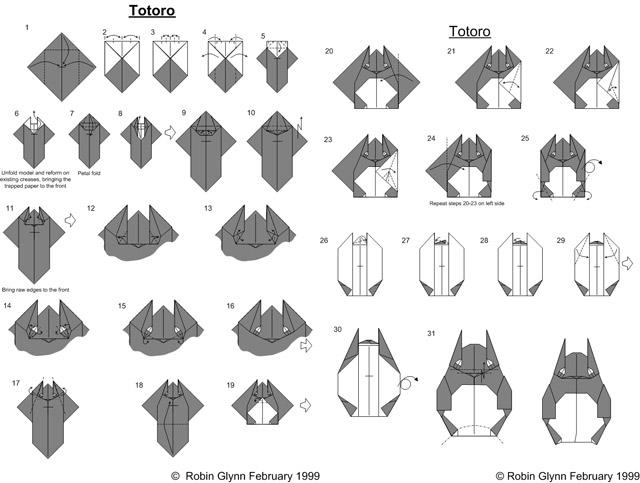
\includegraphics[scale=0.6]{./fig/totoro-origami.jpg}
\caption[Figure caption entry for list of figures]{Figure Caption}
\label{fig:example}		
\end{figure}

% TABLES
% if you have text that needs wrapping, use p{5cm}, in place of l c or r, to set a column width.  Vary the width to find one that fits 

% a small table can often be fitted whole into a file:
\begin{table}[t]
\centering
\caption[Table caption entry for list of tables]{Table Caption}
\label{tab:example1}
\begin{tabular}{lc}
\hline
\textbf{Year} & \textbf{Film Title} \\
\hline
1988 & Grave of the Fireflies \\
1988 & My Neighbour Totoro \\
1994 & Pom Poko \\
2001 & Spirited Away \\
2014 & The Wind Rises \\
\hline
\end{tabular}
\end{table}

% if a table is much larger you can call it from a different file:
\begin{table}[t]
\centering
\caption[Table caption entry for list of tables]{Table Caption}
\label{tab:example2}
%\begin{tabular}{lc}
\hline
\textbf{Fact} & \textbf{Statistic} \\
\hline
My Neighbour Totoro IMDb rating & 8.2 \\
Japan Academy Prizes & 3 \\
Number of feature films & 20 \\
Years since founded & 28 \\
Employees & 300 \\
\hline
\end{tabular}  % this reads in an ugly file containing everything in the tabular environment
\end{table}


% EQUATIONS
\begin{equation} \label{eq:example}
E=mc^{2}
\end{equation}

\begin{equation} \label{eq:calculus}
\frac{df}{dt}=\lim_{h\to0}\frac{f(t+h)-f(t)}{h}
\end{equation}

Inline equations can also be used in the text using dollar signs e.g. $H=-\sum p(x) logp(x)$.

% REFERRING TO FIGURE/TABLE/SECTION/EQUATION LABELS

Use labels to refer to automatic numbering such as with Figure \ref{fig:example}, Table \ref{tab:example1} whilst Tables \ref{tab:example1} and \ref{tab:example2} can be referred to like this which are all found in Chapter \ref{ch:example}.

% CITATIONS
Citation in parantheses: \citep{Soo2011}

Citation in text: \citet{Greenberg2012}

Multiple citations: \citep{Soo2011,Suctani2011,Greenberg2012}







	

!

The text in the curly brackets is the location of the .tex file to be read in.  The \texttt{.} refers to the folder that \textit{Master\_Document.tex} is sitting in (the main folder) and each \texttt{/} is a folder.  So for example, the line above tells \LaTeX{} to look in the \textit{tex} folder for the file \texttt{chapter\_example.tex}.  Copy and Paste this line and change the name of the file for new chapters.  The \texttt{front\_matter} will be described with in Section \ref{sec:front_matter}.

\subsubsection{Making the PDF}
To compile the file and get your PDF in Texmaker, choose the `PDFLaTeX' option from the dropdown menu at the top of the main window and press the arrow to compile it.  To view the PDF, choose `View PDF' from the dropdown menu to the right of the last one and press the arrow button.  When you compile the PDF, a little window should pop at the bottom to tell you how it went, often there will be errors but it does at least tell which file and the line number they occur on!  

It's good idea to compile \textit{Master\_Document.tex} twice in a row. When \LaTeX{} has to make note of the internal document structure it is too too late to actually write it to the PDF...it's weird but that's how it works!  This is often the case for Table of Contents and for citations.

\subsection{Chapters}
Each chapter file begins with \verb!\chapter{}! with the title of your chapter in the curly brackets.  The \verb!\label{}! command allows you give this chapter heading a unique reference which you can use to automatically refer to this chapter number anywhere in the thesis using \verb!\ref{}!.  

\subsubsection{Section Headers and Text}
Section headers work the same way as Chapter titles, you just enter the header text within the curly brackets.  There are three levels of section headers you can use.  

The actual text is just text except when you need to specify any special characters or formatting like italics. Paragraphs are seperated by a space like in word\footnote{This is controlled by the package `parskip' in the \textit{Thesis\_Formatting.sty} file. By default, \LaTeX{} produces a hanging paragraph which you get by commenting out or deleting the parskip package command.}.

\subsubsection{Figures} \label{sec:figures}
Figures have a few lines of special code.  The \verb!\begin{figure}! and \verb!end{figure}! are a special `environment' for figures (often called a float environment).  The \verb!\centering! command center justifies the figure.  The actual figure is inserted using the \verb!includegraphics! command using the location of the figure file. The scale part allows you to scale the size of the figure i.e. 0.5 is half the size.

The \verb!\caption! command automatically adds a figure caption.  Add the caption text in the curly brackets.  If you want a shorter caption to appear in the List of Figures then add this into the square brackets.  Again, the \verb+\label{}+ allows you to give the Figure a unique reference.  \LaTeX{} can tell the difference between labels used for a section and a figure.  The figure will automatically numbered according to where it sits in the chapter file relative to the other figures.  If you decide to change the order of figures, just move this fragment of code to where you want it in the file and \LaTeX{} will take care of changing the numbering in all references to it.

\LaTeX{} has rules about where to place figures and sometimes behaves like Word putting figures in random places.  You can change this by using the \verb![t]! option next to \verb!\begin{figure}!.  The `\texttt{t}' tells \LaTeX{} to put it at the top of a page.  There are other options (see the WikiBook) but this one seemed to be a good default option.

\subsubsection{Tables}
Tables are similar to Figures except sadly way more fiddly!  The caption and label are now at the top but work the same way as with the Figures.  

The \verb!\begin{tabular}{lcc}! command signifies you are inputting the actual table contents.  The \verb!{lcc}! is an instruction for the justification of each column e.g. one left-justified and two center-justified columns.  You can add more.  Then each row of the table is listed using \verb!&! to seperate each column and \verb!\\! to signify the end of the column.

You have now realised Tables are the downfall of \LaTeX!  I reccomend looking at the Wikibook for examples and help with Tables (see Section \ref{sec:resources}).  There are also tools online that can take an excel spreadsheet and format it which saves a lot of time.  The \textit{tab} folder exists so that you can hide away the ugly table contents and work on them separately more easily.  To do this use the \verb!\begin{tabular}{lc}
\hline
\textbf{Fact} & \textbf{Statistic} \\
\hline
My Neighbour Totoro IMDb rating & 8.2 \\
Japan Academy Prizes & 3 \\
Number of feature films & 20 \\
Years since founded & 28 \\
Employees & 300 \\
\hline
\end{tabular}! command as shown in the template.

\subsubsection{Equations}
Equations are again similar to Figures and Tables.  You use the \verb!\begin{equation}! environment and again use a label if you want to refer to the equation by number.  Alternatively, you can use dollar signs `\verb!$!' to put some maths within a sentence like this: \verb!$y=x$!.

There are endless options for equations so see the WikiBook or the cheat-sheet at the back. Texmaker has a lot of support for making equations more quickly.

\subsubsection{Appendices}
Appendices work in the exact same way as the chapter does.  Although it will start with the \verb!\chapter{}! command, \LaTeX{} will interpret it as an Appendix because it's called within an appendix environment in \textit{Master\_Document.tex}.  This means it will write `Appendix...' instead of `Chapter...' at the top and label them A, B, C... rather than 1, 2, 3...

\subsection{Importing Word Files}
So you have your chapter in a Word document and you want to put it into \LaTeX{} but how do you go about it? There might be automatic ways to do this but it doesn't take too long manually (at most a day or two).  I reccomend going about it the following way:

\begin{enumerate}
\item Make a new .tex document and first put the chapter and section headers in.
\item Put the figures and tables in under the relevant sections.  This is often the time when things can go wrong and its easier to figure out what happened without everything else in the document\footnote{Run \LaTeX{} after entering each Figure/Table so you can identify any errors straightaway.}.
\item Copy/Paste the text in\footnote{Go a few paragraphs at a time so you can add formatting, citations and references to labels} and add any equations you have.
\end{enumerate}

\textit{Master\_Document.tex} has the command \verb!\includeonly{./tex/chapter_example}! which when uncommented will produce a PDF with only the chapter(s) selected.  This is quite useful when you are putting together a chapter and don't want to be scrolling through a large PDF document to see any changes you made.

\section{References and Citations}

\subsection{References}
This template is set up with BibTeX which is manages references and citations, similar to EndNote.  The details for each reference you cite are in the \textit{Thesis\_References.bib} file in the main folder which can be opened with the editor.  Each reference has a list of fields like title and authors.  If you have used EndNote or something similar you should be able to export your database as a .bib file!  If you haven't done that (I didn't!), then you can download the formatted information for each paper from the journal online\footnote{Often there is an `Export Citation' button online and you can choose .bib or BibTeX output} and copy it into your own .bib file\footnote{This is a good job for spare half hours when you have lost to the will to continue}.

Each reference has special field at the beginning that acts as a unique identifier that you will use for the citation.  You can choose anything you want for this.  I use the first author name and year e.g. Henson et al. (2012) would be `Henson2012'. 

The reference section is made in the textit{references.tex} file in the \textit{tex} folder.  \verb!\bibliographystyle{}! sets a referencing style which is defined by a file in the main folder. The template has a few different options for styles that have been borrowed from journals. The \verb!\bibliography{}! command then makes the reference section using the .bib file you made.  That's it, it will sort everything else.     

If you have a Mac, you can use free software called BibDesk which shows a database type window like EndNote to help sort your references.  If you have windows, there are other reference managers available such as JabRef (\url{http://jabref.sourceforge.net/index.php}) although I haven't tried them. 

\subsection{Citations}
To cite an article you will mainly use one of two options.  \verb!\citep{Wilson2012}! will insert a citation in brackets e.g. (Wilson et al. 2012) for the paper you labelled as Wilson2012 in the .bib file.  \verb!\citet{Wilson2012}! will do Wilson et al. (2012) instead. Again there are other options if you need them.

\subsection{Running \LaTeX{} with References}
There is one extra step to incorporate the references properly.  In texmaker, choose BibTeX from the drop down menu and click the arrow run button.  You will then have to choose PdfLaTeX again and run it at least once.  You only have to do this additional BibTeX run when you have added citations and references.    

\section{Front Matter} \label{sec:front_matter}
The \textit{Front\_Matter.tex} file in \textit{tex} folder contains everything before the first chapter.  The abstract, a page for notes and acknowledgements are chapters that are left unumbered by the \verb!*!. The declarations are included as a PDF file, taken from the Cardiff Uni website.

\subsection{Title Page}
The title page is in a separate file in the \textit{tex} folder as its not a simple piece of code.  The current title page format was adapted from an example on the WikiBook.  The relevant details can be changed to suit you.

\section{Formatting} \label{sec:formatting}
Tweaking the look and design of the thesis is a little more complicated.  Everything formatting and structure related is found in the \textit{Thesis\_Formatting.sty} file in the main folder.  It has been organised into three main sections.  The first section contains commands to load packages, which are pre-defined bits of code that do specific things.  For example, the parskip package lets \LaTeX{} recognise white-space in the text as a paragraph break (by default you would have hanging paragraphs).  If you want to do something specific in your thesis, google it and most likely someone will have made a package. The second section contains common one-off user options.  The third section contains the main formatting options.  Each option usually has an associated package followed by some options.  I've tried to lay out common things like header font options so you can play around with them as well as providing links for more information.

\section{Resources} \label{sec:resources}

\begin{itemize}
\item This wikibook covers almost everything you would want to know: \url{http://en.wikibooks.org/wiki/LaTeX}

\item Google! Someone somewhere will have asked that question online and got an answer.  Often there are more than one way of doing things so copy/paste bits of code and see what happens.  If you don't like you can just re-compile your document without it and it will be the same as before!  

\item Cheat Sheet: A cheat sheet is attached on the next page which is a quick reference for the commonly used elements of \LaTeX{}.

\item The Graduate College runs workshops on \LaTeX{} which are really good for an introduction.

\item MOOCs: Have a look round for free online courses for \LaTeX{}.  The Coursera MOOC (\url{https://www.coursera.org/}) only has one in Russian but might be likely to have one in the future.

\end{itemize}


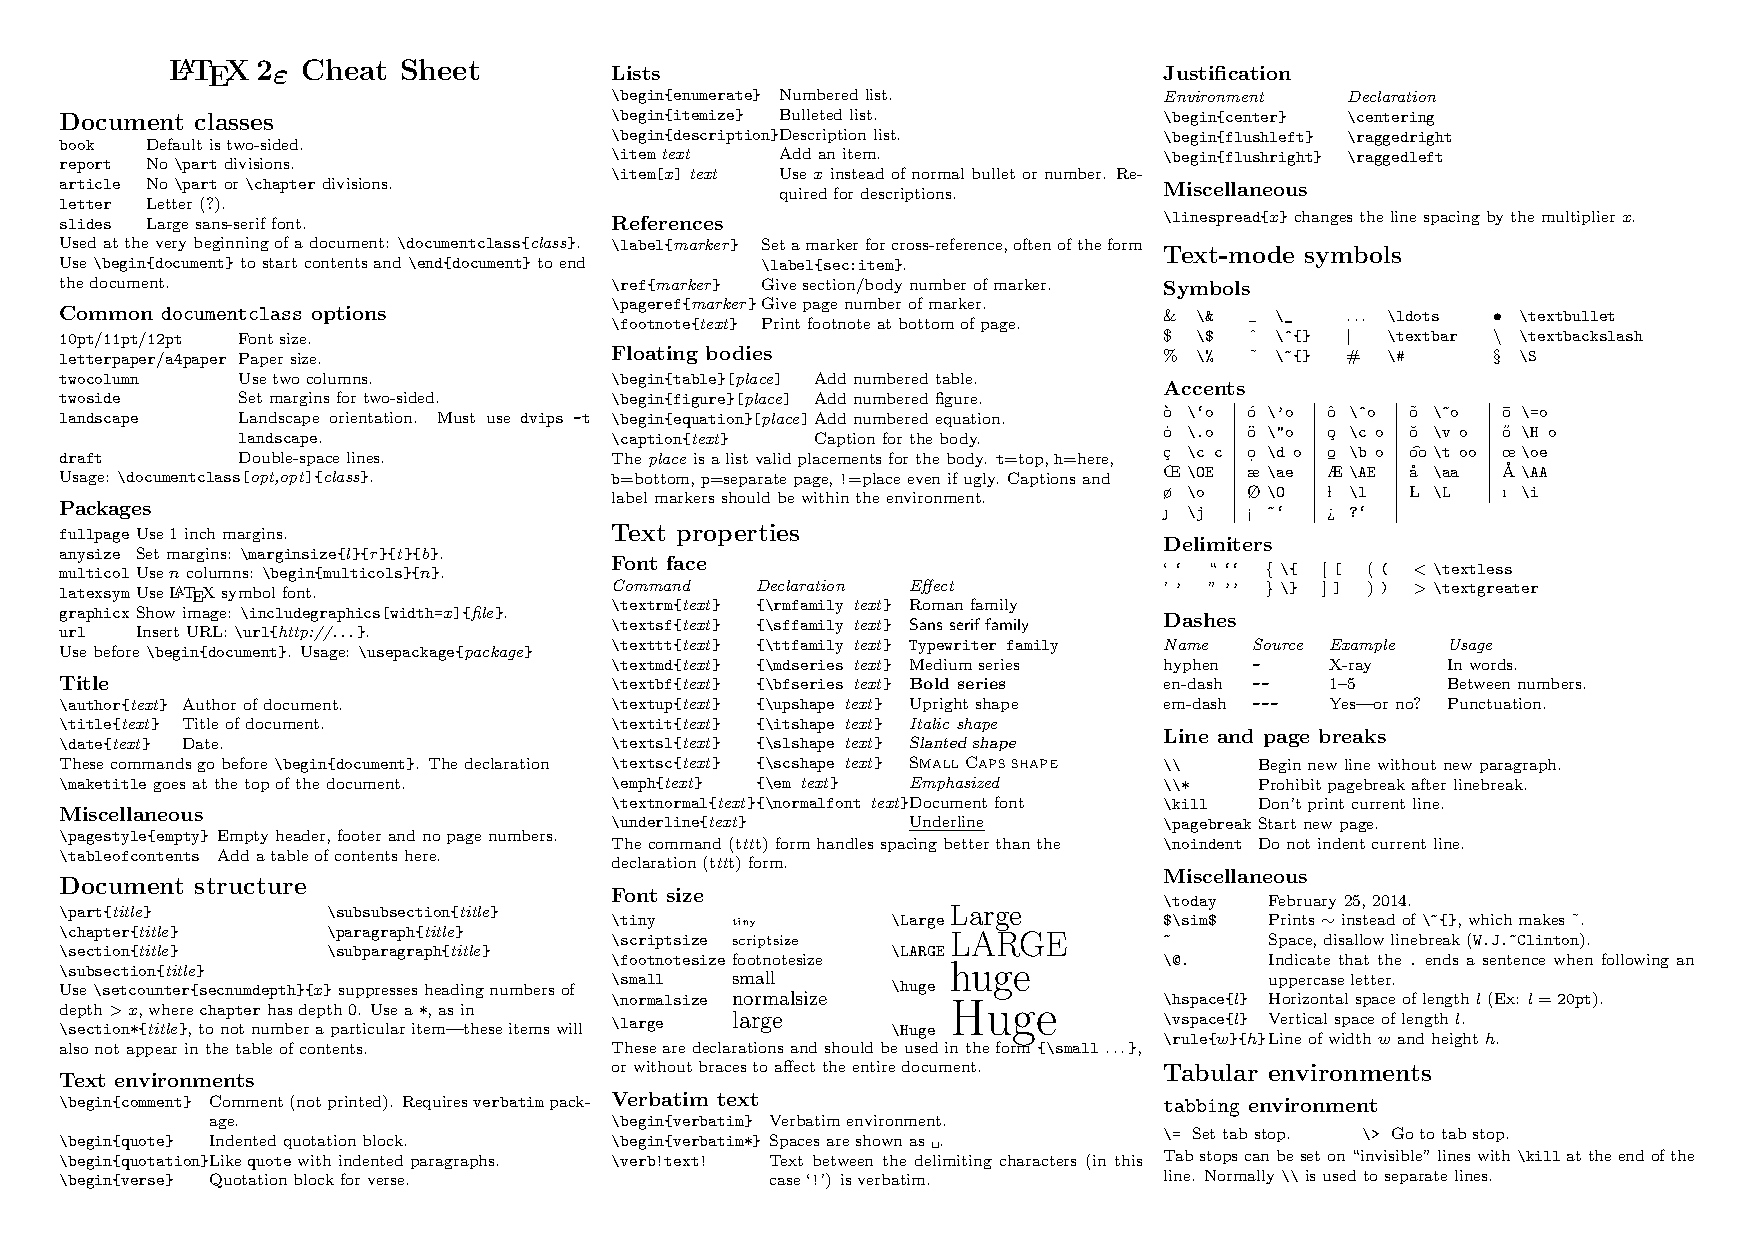
\includepdf[pages=-,landscape=true]{cheat_sheet.pdf}


\end{document}